% ===========================================================================
%  TikuOS — Bus Interfaces: I2C & SPI
%  Beamer Presentation
% ===========================================================================
\documentclass[aspectratio=169, 10pt]{beamer}

% ---- Theme ----------------------------------------------------------------
\usetheme{Madrid}
\usecolortheme{whale}
\setbeamertemplate{navigation symbols}{}
\setbeamertemplate{footline}{%
  \leavevmode\hbox{%
    \begin{beamercolorbox}[wd=.33\paperwidth,ht=2.5ex,dp=1ex,center]{author in head/foot}%
      \usebeamerfont{author in head/foot}\insertshortauthor
    \end{beamercolorbox}%
    \begin{beamercolorbox}[wd=.34\paperwidth,ht=2.5ex,dp=1ex,center]{title in head/foot}%
      \usebeamerfont{title in head/foot}\insertshorttitle
    \end{beamercolorbox}%
    \begin{beamercolorbox}[wd=.33\paperwidth,ht=2.5ex,dp=1ex,right]{date in head/foot}%
      \usebeamerfont{date in head/foot}\insertshortdate{}\hspace*{2em}%
      \insertframenumber{}/\inserttotalframenumber\hspace*{2ex}
    \end{beamercolorbox}}%
  \vskip0pt%
}

% ---- Packages -------------------------------------------------------------
\usepackage{listings}
\usepackage{graphicx}
\usepackage{hyperref}
\usepackage{booktabs}
\usepackage{multirow}
\usepackage{tikz}
\usetikzlibrary{arrows.meta, positioning, shapes.geometric, calc,
                decorations.pathreplacing, fit}

% ---- Code listing style ---------------------------------------------------
\lstset{
  basicstyle=\ttfamily\scriptsize,
  keywordstyle=\color{blue}\bfseries,
  commentstyle=\color{gray},
  stringstyle=\color{red!70!black},
  showstringspaces=false,
  breaklines=true,
  frame=single,
  rulecolor=\color{black!30},
  backgroundcolor=\color{blue!3},
  tabsize=4,
}
\lstdefinestyle{cstyle}{
  language=C,
  morekeywords={uint8_t,uint16_t,uint32_t,int8_t,
                tiku_i2c_config_t,tiku_spi_config_t,
                TIKU_I2C_OK,TIKU_I2C_ERR_NACK,
                TIKU_I2C_ERR_TIMEOUT,TIKU_I2C_ERR_PARAM,
                TIKU_I2C_SPEED_STANDARD,TIKU_I2C_SPEED_FAST,
                TIKU_SPI_OK,TIKU_SPI_ERR_TIMEOUT,TIKU_SPI_ERR_PARAM,
                TIKU_SPI_MODE_0,TIKU_SPI_MODE_1,
                TIKU_SPI_MODE_2,TIKU_SPI_MODE_3,
                TIKU_SPI_MSB_FIRST,TIKU_SPI_LSB_FIRST,
                TIKU_BOARD_SPI_BRW_1MHZ,TIKU_BOARD_SPI_BRW_4MHZ,
                TIKU_BOARD_SPI_BRW_2MHZ,TIKU_BOARD_SPI_BRW_500KHZ,
                TIKU_BOARD_I2C_BRW_100K,TIKU_BOARD_I2C_BRW_400K,
                TIKU_BOARD_I2C_PINS_INIT,TIKU_BOARD_SPI_PINS_INIT,
                TIKU_PROCESS,TIKU_PROCESS_THREAD,
                TIKU_PROCESS_BEGIN,TIKU_PROCESS_END,
                TIKU_PROCESS_WAIT_EVENT,TIKU_PROCESS_WAIT_EVENT_UNTIL,
                TIKU_AUTOSTART_PROCESSES,TIKU_EVENT_TIMER,
                NULL},
}

% ---- Metadata -------------------------------------------------------------
\title[TikuOS Bus Interfaces]{TikuOS Bus Interfaces: I2C \& SPI}
\subtitle{Simple. Ubiquitous. Intelligence, Everywhere.}
\author[Ambuj Varshney]{Ambuj Varshney \\ \texttt{ambuj@tiku-os.org}}
\date{\today}

% ===========================================================================
\begin{document}

% ---------------------------------------------------------------------------
\begin{frame}
\titlepage
\end{frame}

% ---------------------------------------------------------------------------
\begin{frame}{Outline}
\tableofcontents
\end{frame}

% ===========================================================================
\section{Architecture Overview}
% ===========================================================================

\begin{frame}[fragile]{Three-Layer Bus Abstraction}
\begin{center}
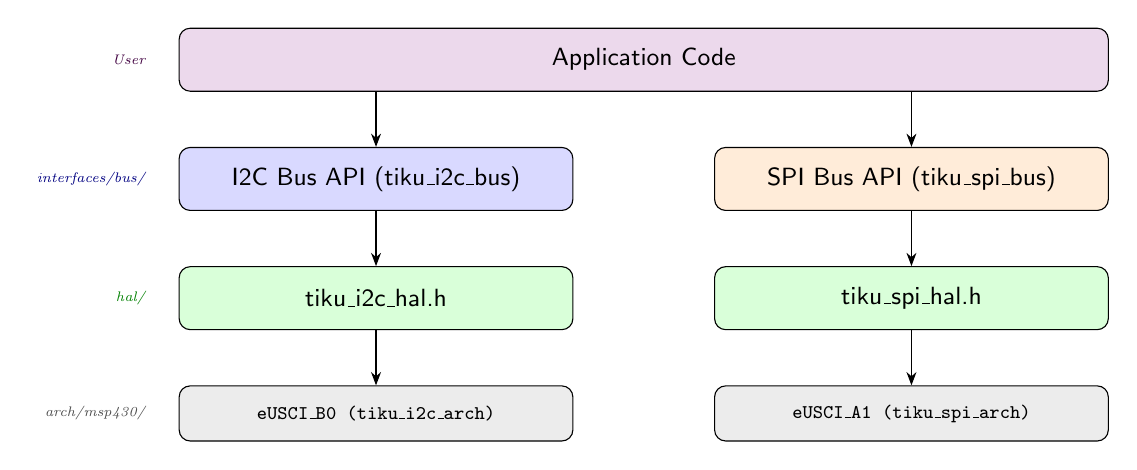
\begin{tikzpicture}[
    box/.style={draw, rounded corners, minimum height=0.8cm,
                text centered, font=\small\sffamily, fill=#1},
    hw/.style={draw, rounded corners, minimum height=0.7cm,
               text centered, font=\scriptsize\ttfamily, fill=gray!15},
    >=Stealth, node distance=0.5cm
  ]

  % Application layer
  \node[box=violet!15, minimum width=11.8cm] (app)
    {Application Code};

  % Bus API layer
  \node[box=blue!15, minimum width=5cm, below=0.7cm of app.south west,
        anchor=north west] (i2c_api)
    {I2C Bus API (tiku\_i2c\_bus)};
  \node[box=orange!15, minimum width=5cm, below=0.7cm of app.south east,
        anchor=north east] (spi_api)
    {SPI Bus API (tiku\_spi\_bus)};

  % HAL layer
  \node[box=green!15, minimum width=5cm, below=0.7cm of i2c_api] (i2c_hal)
    {tiku\_i2c\_hal.h};
  \node[box=green!15, minimum width=5cm, below=0.7cm of spi_api] (spi_hal)
    {tiku\_spi\_hal.h};

  % Arch layer
  \node[hw, minimum width=5cm, below=0.7cm of i2c_hal] (i2c_arch)
    {eUSCI\_B0 (tiku\_i2c\_arch)};
  \node[hw, minimum width=5cm, below=0.7cm of spi_hal] (spi_arch)
    {eUSCI\_A1 (tiku\_spi\_arch)};

  % Arrows
  \draw[->] (app.south -| i2c_api.north) -- (i2c_api);
  \draw[->] (app.south -| spi_api.north) -- (spi_api);
  \draw[->] (i2c_api) -- (i2c_hal);
  \draw[->] (spi_api) -- (spi_hal);
  \draw[->] (i2c_hal) -- (i2c_arch);
  \draw[->] (spi_hal) -- (spi_arch);

  % Labels
  \node[left=0.3cm of app, font=\tiny\itshape, text=violet!50!black] {User};
  \node[left=0.3cm of i2c_api, font=\tiny\itshape, text=blue!50!black]
    {interfaces/bus/};
  \node[left=0.3cm of i2c_hal, font=\tiny\itshape, text=green!50!black]
    {hal/};
  \node[left=0.3cm of i2c_arch, font=\tiny\itshape, text=gray!60!black]
    {arch/msp430/};

\end{tikzpicture}
\end{center}

\vspace{0.3em}
\begin{alertblock}{Design Principle}
Platform-independent API in \texttt{interfaces/bus/}.
Board-specific pin routing and clock prescalers in board headers.
One arch implementation works across all MSP430FR variants.
\end{alertblock}
\end{frame}

% ---------------------------------------------------------------------------
\begin{frame}{I2C vs SPI at a Glance}
\begin{table}
\centering
\small
\begin{tabular}{@{}lll@{}}
\toprule
& \textbf{I2C} & \textbf{SPI} \\
\midrule
Wires         & 2 (SDA + SCL) & 3 + 1/device (SCLK + SIMO + SOMI + CS) \\
Addressing    & 7-bit slave address on bus & Chip select GPIO per device \\
Duplex        & Half-duplex & Full-duplex \\
Speed         & 100\,kHz / 400\,kHz & Up to SMCLK/2 (4\,MHz @ 8\,MHz) \\
MSP430 Module & eUSCI\_B0 & eUSCI\_A1 \\
Typical Use   & Sensors, EEPROMs, RTCs & Flash, displays, radio transceivers \\
\bottomrule
\end{tabular}
\end{table}

\vspace{0.5em}
\begin{columns}[T]
\begin{column}{0.48\textwidth}
\begin{block}{FR5969 LaunchPad I2C Pins}
P1.6 = SDA, P1.7 = SCL\\
(eUSCI\_B0, SEL1=1 SEL0=0)
\end{block}
\end{column}
\begin{column}{0.48\textwidth}
\begin{block}{FR5969 LaunchPad SPI Pins}
P2.5 = CLK, P2.6 = SIMO, P2.7 = SOMI\\
(eUSCI\_A1, SEL1=1 SEL0=0)
\end{block}
\end{column}
\end{columns}
\end{frame}

% ===========================================================================
\section{I2C Bus Interface}
% ===========================================================================

% ---------------------------------------------------------------------------
\subsection{I2C Protocol}

\begin{frame}[fragile]{I2C Protocol Basics}
\begin{center}
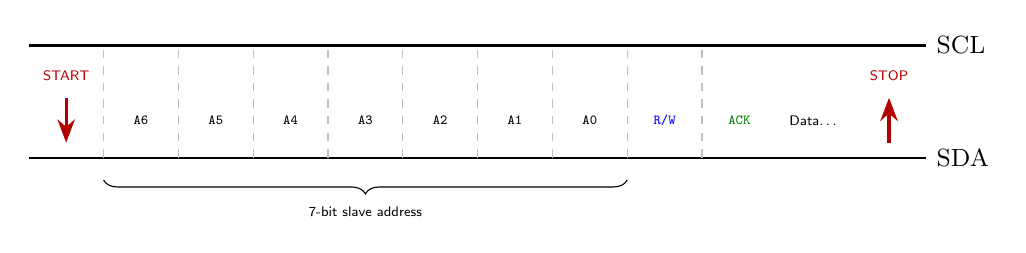
\begin{tikzpicture}[>=Stealth, scale=0.95]
  % Bus lines
  \draw[thick] (0,1.5) -- (12,1.5) node[right, font=\small] {SCL};
  \draw[thick] (0,0) -- (12,0) node[right, font=\small] {SDA};

  % START condition
  \draw[red!70!black, very thick, ->] (0.5,0.8) -- (0.5,0.2);
  \node[above, font=\tiny\sffamily, red!70!black] at (0.5,0.9) {START};

  % Address bits (7)
  \foreach \i/\b in {1/A6, 2/A5, 3/A4, 4/A3, 5/A2, 6/A1, 7/A0} {
    \node[font=\tiny\ttfamily] at (\i+0.5, 0.5) {\b};
    \draw[gray!50, dashed] (\i,0) -- (\i,1.5);
  }
  % R/W bit
  \node[font=\tiny\ttfamily, blue] at (8.5, 0.5) {R/W};
  \draw[gray!50, dashed] (8,0) -- (8,1.5);

  % ACK
  \node[font=\tiny\ttfamily, green!50!black] at (9.5, 0.5) {ACK};
  \draw[gray!50, dashed] (9,0) -- (9,1.5);

  % Data
  \node[font=\tiny\sffamily] at (10.5, 0.5) {Data\dots};

  % STOP condition
  \draw[red!70!black, very thick, ->] (11.5,0.2) -- (11.5,0.8);
  \node[above, font=\tiny\sffamily, red!70!black] at (11.5,0.9) {STOP};

  % Braces
  \draw[decorate, decoration={brace, amplitude=5pt, mirror}]
    (1,-0.3) -- (8,-0.3) node[midway, below=6pt, font=\tiny\sffamily]
    {7-bit slave address};
\end{tikzpicture}
\end{center}

\vspace{0.3em}
\begin{columns}[T]
\begin{column}{0.48\textwidth}
\textbf{Transaction types:}
\begin{itemize}
  \item \textbf{Write}: START $\rightarrow$ addr+W $\rightarrow$ data $\rightarrow$ STOP
  \item \textbf{Read}: START $\rightarrow$ addr+R $\rightarrow$ data $\rightarrow$ NACK $\rightarrow$ STOP
  \item \textbf{Write-Read}: write $\rightarrow$ repeated START $\rightarrow$ read
        (register-read pattern)
\end{itemize}
\end{column}
\begin{column}{0.48\textwidth}
\textbf{Key characteristics:}
\begin{itemize}
  \item Multi-master, multi-slave on same bus
  \item ACK/NACK feedback per byte
  \item Clock stretching by slave
  \item Open-drain lines with pull-ups
\end{itemize}
\end{column}
\end{columns}
\end{frame}

% ---------------------------------------------------------------------------
\subsection{I2C API}

\begin{frame}[fragile]{I2C Configuration \& Status Codes}
\begin{columns}[T]
\begin{column}{0.48\textwidth}
\begin{lstlisting}[style=cstyle,
  title={interfaces/bus/tiku\_i2c\_bus.h}]
/* Speed modes */
#define TIKU_I2C_SPEED_STANDARD 0
#define TIKU_I2C_SPEED_FAST     1

/* Status codes */
#define TIKU_I2C_OK           0
#define TIKU_I2C_ERR_NACK   (-1)
#define TIKU_I2C_ERR_TIMEOUT (-2)
#define TIKU_I2C_ERR_BUSY   (-3)
#define TIKU_I2C_ERR_PARAM  (-4)

/* Configuration */
typedef struct tiku_i2c_config {
    uint8_t speed;
} tiku_i2c_config_t;
\end{lstlisting}
\end{column}

\begin{column}{0.48\textwidth}
\textbf{Speed modes:}
\begin{itemize}
  \item \texttt{STANDARD}: 100\,kHz (prescaler 80)
  \item \texttt{FAST}: 400\,kHz (prescaler 20)
  \item Prescalers from 8\,MHz SMCLK
\end{itemize}

\vspace{0.5em}
\begin{block}{Error Handling}
Every bus operation returns a status code.\\
\texttt{NACK}: slave didn't respond --- wrong address or busy.\\
\texttt{TIMEOUT}: bus stuck --- hardware issue.\\
All errors auto-issue STOP to release bus.
\end{block}
\end{column}
\end{columns}
\end{frame}

% ---------------------------------------------------------------------------
\begin{frame}[fragile]{I2C API Functions}
\begin{table}
\centering
\small
\begin{tabular}{@{}lp{8cm}@{}}
\toprule
\textbf{Function} & \textbf{Description} \\
\midrule
\texttt{tiku\_i2c\_init(config)}    & Initialize eUSCI\_B0 in I2C master mode \\
\texttt{tiku\_i2c\_close()}         & Place peripheral in reset \\
\midrule
\texttt{tiku\_i2c\_write(addr, buf, len)}
    & START $\rightarrow$ addr+W $\rightarrow$ data $\rightarrow$ STOP \\
\texttt{tiku\_i2c\_read(addr, buf, len)}
    & START $\rightarrow$ addr+R $\rightarrow$ data $\rightarrow$ NACK $\rightarrow$ STOP \\
\texttt{tiku\_i2c\_write\_read(addr, tx, tx\_len, rx, rx\_len)}
    & Write then repeated-START read (register access) \\
\bottomrule
\end{tabular}
\end{table}

\vspace{0.3em}
\begin{lstlisting}[style=cstyle, title={Typical register-read pattern}]
/* Read 2 bytes from register 0x05 of device at address 0x48 */
uint8_t reg = 0x05;
uint8_t buf[2];
int rc = tiku_i2c_write_read(0x48, &reg, 1, buf, 2);
if (rc != TIKU_I2C_OK) {
    /* handle error */
}
\end{lstlisting}
\end{frame}

% ---------------------------------------------------------------------------
\subsection{I2C Architecture}

\begin{frame}[fragile]{I2C Board \& Device Macros}
\begin{columns}[T]
\begin{column}{0.48\textwidth}
\begin{lstlisting}[style=cstyle,
  title={devices/tiku\_device\_fr5969.h}]
/* eUSCI peripheral availability */
#define TIKU_DEVICE_HAS_EUSCIB0 1
#define TIKU_DEVICE_HAS_EUSCIB1 1
\end{lstlisting}

\begin{lstlisting}[style=cstyle,
  title={boards/tiku\_board\_fr5969\_launchpad.h}]
/* I2C on eUSCI_B0:
   P1.6 = SDA, P1.7 = SCL */
#define TIKU_BOARD_I2C_PINS_INIT() \
    do { P1SEL1 |= BIT6 | BIT7; \
         P1SEL0 &= ~(BIT6 | BIT7);\
    } while(0)

/* Prescalers from 8 MHz SMCLK */
#define TIKU_BOARD_I2C_BRW_100K 80
#define TIKU_BOARD_I2C_BRW_400K 20
\end{lstlisting}
\end{column}

\begin{column}{0.48\textwidth}
\textbf{Adding a new board:}
\begin{enumerate}
  \item Create board header in \texttt{boards/}
  \item Define \texttt{TIKU\_BOARD\_I2C\_PINS\_INIT()}
        with correct port and pin SEL bits
  \item Define prescaler macros for the board's
        SMCLK frequency
  \item Add \texttt{\#elif} in \texttt{tiku\_device\_select.h}
\end{enumerate}

\vspace{0.5em}
\begin{block}{Pin Function Select}
MSP430FR5969 uses SEL1:SEL0 = 1:0 for
eUSCI\_B0 alternate function on P1.6/P1.7.
\end{block}
\end{column}
\end{columns}
\end{frame}

% ---------------------------------------------------------------------------
\begin{frame}[fragile]{I2C Arch: Initialization}
\begin{lstlisting}[style=cstyle, title={arch/msp430/tiku\_i2c\_arch.c --- tiku\_i2c\_arch\_init()}]
int tiku_i2c_arch_init(const tiku_i2c_config_t *config)
{
    /* Select I2C function on board-specific SDA/SCL pins */
    TIKU_BOARD_I2C_PINS_INIT();

    /* Put eUSCI_B0 in reset before configuration */
    UCB0CTLW0 = UCSWRST;

    /* I2C master mode, synchronous, SMCLK source */
    UCB0CTLW0 |= UCMODE_3 | UCMST | UCSSEL__SMCLK | UCSYNC;

    /* Set clock prescaler for requested speed */
    if (config->speed == TIKU_I2C_SPEED_FAST) {
        UCB0BRW = TIKU_BOARD_I2C_BRW_400K;
    } else {
        UCB0BRW = TIKU_BOARD_I2C_BRW_100K;
    }

    UCB0CTLW1 = UCASTP_0;       /* Manual STOP (no auto-stop) */
    UCB0CTLW0 &= ~UCSWRST;      /* Release from reset */
    return TIKU_I2C_OK;
}
\end{lstlisting}
\end{frame}

% ---------------------------------------------------------------------------
\begin{frame}[fragile]{I2C Arch: Write \& Read}
\begin{columns}[T]
\begin{column}{0.48\textwidth}
\begin{lstlisting}[style=cstyle, basicstyle=\ttfamily\tiny,
  title={Write transaction}]
int tiku_i2c_arch_write(
    uint8_t addr,
    const uint8_t *buf, uint16_t len)
{
    UCB0I2CSA = addr;
    UCB0CTLW0 |= UCTR | UCTXSTT;

    for (i = 0; i < len; i++) {
        rc = i2c_wait_flag(UCTXIFG0);
        if (rc != TIKU_I2C_OK)
            return rc;
        UCB0TXBUF = buf[i];
    }

    /* Wait for last byte */
    rc = i2c_wait_flag(UCTXIFG0);
    if (rc != TIKU_I2C_OK)
        return rc;

    UCB0CTLW0 |= UCTXSTP;
    return i2c_wait_stop();
}
\end{lstlisting}
\end{column}

\begin{column}{0.48\textwidth}
\begin{lstlisting}[style=cstyle, basicstyle=\ttfamily\tiny,
  title={Read transaction (multi-byte)}]
int tiku_i2c_arch_read(
    uint8_t addr,
    uint8_t *buf, uint16_t len)
{
    UCB0I2CSA = addr;
    UCB0CTLW0 &= ~UCTR;
    UCB0CTLW0 |= UCTXSTT;

    for (i = 0; i < len; i++) {
        /* STOP before last byte */
        if (i == len - 1)
            UCB0CTLW0 |= UCTXSTP;

        rc = i2c_wait_flag(UCRXIFG0);
        if (rc != TIKU_I2C_OK)
            return rc;
        buf[i] = (uint8_t)UCB0RXBUF;
    }

    return i2c_wait_stop();
}
\end{lstlisting}

\vspace{0.3em}
\begin{alertblock}{Single-Byte Read}
For \texttt{len==1}, STOP must be issued
right after the address phase completes
(special handling in the driver).
\end{alertblock}
\end{column}
\end{columns}
\end{frame}

% ---------------------------------------------------------------------------
\begin{frame}[fragile]{I2C Arch: Timeout \& NACK Detection}
\begin{lstlisting}[style=cstyle, title={Timeout-guarded flag wait with NACK detection}]
static int i2c_wait_flag(uint16_t flag)
{
    uint16_t timeout = 10000U;

    while (!(UCB0IFG & flag)) {
        if (UCB0IFG & UCNACKIFG) {       /* Slave NACKed */
            UCB0IFG &= ~UCNACKIFG;
            UCB0CTLW0 |= UCTXSTP;        /* Issue STOP to release bus */
            while (UCB0CTLW0 & UCTXSTP);
            return TIKU_I2C_ERR_NACK;
        }
        if (--timeout == 0) {
            UCB0CTLW0 |= UCTXSTP;        /* Force STOP on timeout */
            return TIKU_I2C_ERR_TIMEOUT;
        }
    }
    return TIKU_I2C_OK;
}
\end{lstlisting}

\vspace{0.3em}
\begin{block}{Bus Recovery}
Every error path issues a STOP condition to release SDA/SCL,
preventing bus lockup. The timeout counter (\textasciitilde10\,000 iterations
at 8\,MHz $\approx$ 1\,ms) guards against stuck-bus scenarios.
\end{block}
\end{frame}

% ===========================================================================
\section{SPI Bus Interface}
% ===========================================================================

% ---------------------------------------------------------------------------
\subsection{SPI Protocol}

\begin{frame}[fragile]{SPI Protocol Basics}
\begin{center}
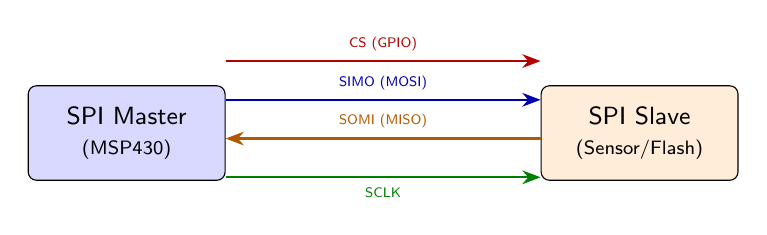
\begin{tikzpicture}[
    box/.style={draw, rounded corners=3pt, minimum height=1.2cm,
                minimum width=2.5cm, align=center, font=\small\sffamily},
    >=Stealth
  ]

  % Master and Slave
  \node[box, fill=blue!15] (master) {SPI Master\\{\scriptsize (MSP430)}};
  \node[box, fill=orange!15, right=4cm of master] (slave) {SPI Slave\\{\scriptsize (Sensor/Flash)}};

  % Signal lines
  \draw[->, thick, blue!70!black]
    ([yshift=12pt]master.east) -- node[above, font=\tiny\sffamily] {SIMO (MOSI)}
    ([yshift=12pt]slave.west);
  \draw[->, thick, orange!70!black]
    ([yshift=-2pt]slave.west) -- node[above, font=\tiny\sffamily] {SOMI (MISO)}
    ([yshift=-2pt]master.east);
  \draw[->, thick, green!50!black]
    ([yshift=-16pt]master.east) -- node[below, font=\tiny\sffamily] {SCLK}
    ([yshift=-16pt]slave.west);

  % CS line
  \draw[->, thick, red!70!black]
    ([yshift=26pt]master.east) -- node[above, font=\tiny\sffamily] {CS (GPIO)}
    ([yshift=26pt]slave.west);

\end{tikzpicture}
\end{center}

\vspace{0.3em}
\begin{columns}[T]
\begin{column}{0.48\textwidth}
\textbf{Four SPI clock modes:}
\begin{table}
\centering
\scriptsize
\begin{tabular}{@{}cccl@{}}
\toprule
\textbf{Mode} & \textbf{CPOL} & \textbf{CPHA} & \textbf{Sampling Edge} \\
\midrule
0 & 0 & 0 & Rising (most common) \\
1 & 0 & 1 & Falling \\
2 & 1 & 0 & Falling \\
3 & 1 & 1 & Rising \\
\bottomrule
\end{tabular}
\end{table}
\end{column}

\begin{column}{0.48\textwidth}
\textbf{Key characteristics:}
\begin{itemize}
  \item Full-duplex: TX and RX simultaneous
  \item No addressing --- CS selects device
  \item No ACK/NACK feedback
  \item Master always generates clock
  \item Much faster than I2C
\end{itemize}
\end{column}
\end{columns}
\end{frame}

% ---------------------------------------------------------------------------
\subsection{SPI API}

\begin{frame}[fragile]{SPI Configuration}
\begin{columns}[T]
\begin{column}{0.48\textwidth}
\begin{lstlisting}[style=cstyle,
  title={interfaces/bus/tiku\_spi\_bus.h}]
/* Clock modes */
#define TIKU_SPI_MODE_0  0
#define TIKU_SPI_MODE_1  1
#define TIKU_SPI_MODE_2  2
#define TIKU_SPI_MODE_3  3

/* Bit order */
#define TIKU_SPI_MSB_FIRST  0
#define TIKU_SPI_LSB_FIRST  1

/* Status codes */
#define TIKU_SPI_OK           0
#define TIKU_SPI_ERR_TIMEOUT (-1)
#define TIKU_SPI_ERR_PARAM   (-2)

typedef struct tiku_spi_config {
    uint8_t  mode;
    uint8_t  bit_order;
    uint16_t prescaler;
} tiku_spi_config_t;
\end{lstlisting}
\end{column}

\begin{column}{0.48\textwidth}
\textbf{Prescaler convenience macros:}\\
(from \texttt{tiku\_board\_fr5969\_launchpad.h})

\vspace{0.3em}
\begin{table}
\centering
\small
\begin{tabular}{@{}lr@{}}
\toprule
\textbf{Macro} & \textbf{SPI Clock} \\
\midrule
\texttt{TIKU\_BOARD\_SPI\_BRW\_4MHZ}   & 4\,MHz \\
\texttt{TIKU\_BOARD\_SPI\_BRW\_2MHZ}   & 2\,MHz \\
\texttt{TIKU\_BOARD\_SPI\_BRW\_1MHZ}   & 1\,MHz \\
\texttt{TIKU\_BOARD\_SPI\_BRW\_500KHZ} & 500\,kHz \\
\bottomrule
\end{tabular}
\end{table}

\vspace{0.3em}
All derived from 8\,MHz SMCLK:\\
\texttt{SPI\_CLK = SMCLK / prescaler}

\vspace{0.3em}
\begin{block}{Chip Select}
CS is managed by the application via GPIO,
not by the SPI driver. This supports
arbitrary CS pin assignment and multi-device buses.
\end{block}
\end{column}
\end{columns}
\end{frame}

% ---------------------------------------------------------------------------
\begin{frame}[fragile]{SPI API Functions}
\begin{table}
\centering
\small
\begin{tabular}{@{}lp{8cm}@{}}
\toprule
\textbf{Function} & \textbf{Description} \\
\midrule
\texttt{tiku\_spi\_init(config)}    & Initialize eUSCI\_A1 in 3-pin SPI master mode \\
\texttt{tiku\_spi\_close()}         & Place peripheral in reset \\
\midrule
\texttt{tiku\_spi\_transfer(byte)}
    & Single-byte full-duplex exchange (returns RX byte) \\
\texttt{tiku\_spi\_write(buf, len)}
    & Bulk write; received data is discarded \\
\texttt{tiku\_spi\_read(buf, len)}
    & Bulk read; sends 0xFF as dummy data \\
\texttt{tiku\_spi\_write\_read(tx, rx, len)}
    & Bulk full-duplex simultaneous TX and RX \\
\bottomrule
\end{tabular}
\end{table}

\vspace{0.3em}
\begin{lstlisting}[style=cstyle, title={Typical SPI device interaction}]
/* Assert CS, send command, read response, deassert CS */
P3OUT &= ~BIT0;                     /* CS low (active) */
tiku_spi_write(cmd, sizeof(cmd));   /* Send command bytes */
tiku_spi_read(response, 4);         /* Read 4 bytes (sends 0xFF) */
P3OUT |= BIT0;                      /* CS high (inactive) */
\end{lstlisting}
\end{frame}

% ---------------------------------------------------------------------------
\subsection{SPI Architecture}

\begin{frame}[fragile]{SPI Board Macros \& Mode Mapping}
\begin{columns}[T]
\begin{column}{0.48\textwidth}
\begin{lstlisting}[style=cstyle,
  title={boards/tiku\_board\_fr5969\_launchpad.h}]
/* SPI on eUSCI_A1:
   P2.5=CLK P2.6=SIMO P2.7=SOMI */
#define TIKU_BOARD_SPI_PINS_INIT() \
    do { \
        P2SEL1 |= BIT5|BIT6|BIT7; \
        P2SEL0 &= ~(BIT5|BIT6|BIT7);\
    } while(0)

/* Prescalers: 8 MHz SMCLK */
#define TIKU_BOARD_SPI_BRW_4MHZ   2
#define TIKU_BOARD_SPI_BRW_2MHZ   4
#define TIKU_BOARD_SPI_BRW_1MHZ   8
#define TIKU_BOARD_SPI_BRW_500KHZ 16
\end{lstlisting}
\end{column}

\begin{column}{0.48\textwidth}
\textbf{MSP430 SPI mode mapping:}

\vspace{0.3em}
MSP430's \texttt{UCCKPH} is \textbf{inverted} relative to
the standard CPHA definition.

\vspace{0.3em}
\begin{table}
\centering
\scriptsize
\begin{tabular}{@{}cccc@{}}
\toprule
\textbf{SPI Mode} & \textbf{UCCKPL} & \textbf{UCCKPH} & \textbf{Bits} \\
\midrule
Mode 0 & 0 & 1 & \texttt{UCCKPH} \\
Mode 1 & 0 & 0 & \texttt{0} \\
Mode 2 & 1 & 1 & \texttt{UCCKPH|UCCKPL} \\
Mode 3 & 1 & 0 & \texttt{UCCKPL} \\
\bottomrule
\end{tabular}
\end{table}

\vspace{0.3em}
\begin{alertblock}{Common Pitfall}
Standard CPHA=0 maps to MSP430 UCCKPH=1.
The driver handles this mapping internally ---
just use \texttt{TIKU\_SPI\_MODE\_0..3}.
\end{alertblock}
\end{column}
\end{columns}
\end{frame}

% ---------------------------------------------------------------------------
\begin{frame}[fragile]{SPI Arch: Initialization}
\begin{lstlisting}[style=cstyle, title={arch/msp430/tiku\_spi\_arch.c --- tiku\_spi\_arch\_init()}]
int tiku_spi_arch_init(const tiku_spi_config_t *config)
{
    /* Select SPI function on board-specific SCLK/SIMO/SOMI pins */
    TIKU_BOARD_SPI_PINS_INIT();

    /* Put eUSCI_A1 in reset before configuration */
    UCA1CTLW0 = UCSWRST;

    /* SPI master, synchronous, 3-pin mode, SMCLK source */
    UCA1CTLW0 |= UCMST | UCSYNC | UCMODE_0 | UCSSEL__SMCLK;

    /* Set clock polarity and phase for requested SPI mode */
    UCA1CTLW0 |= spi_mode_to_bits(config->mode);

    /* Set bit order */
    if (config->bit_order == TIKU_SPI_MSB_FIRST)
        UCA1CTLW0 |= UCMSB;

    /* Set clock prescaler */
    UCA1BRW = config->prescaler;

    UCA1CTLW0 &= ~UCSWRST;  /* Release from reset */
    return TIKU_SPI_OK;
}
\end{lstlisting}
\end{frame}

% ---------------------------------------------------------------------------
\begin{frame}[fragile]{SPI Arch: Transfer Operations}
\begin{columns}[T]
\begin{column}{0.48\textwidth}
\begin{lstlisting}[style=cstyle, basicstyle=\ttfamily\tiny,
  title={Single-byte full-duplex exchange}]
static uint8_t spi_xfer_byte(uint8_t tx)
{
    uint16_t timeout;

    timeout = SPI_TIMEOUT;
    while (!(UCA1IFG & UCTXIFG)) {
        if (--timeout == 0)
            return 0;
    }
    UCA1TXBUF = tx;

    timeout = SPI_TIMEOUT;
    while (!(UCA1IFG & UCRXIFG)) {
        if (--timeout == 0)
            return 0;
    }
    return (uint8_t)UCA1RXBUF;
}
\end{lstlisting}
\end{column}

\begin{column}{0.48\textwidth}
\begin{lstlisting}[style=cstyle, basicstyle=\ttfamily\tiny,
  title={Bulk read (sends 0xFF dummy)}]
int tiku_spi_arch_read(
    uint8_t *buf, uint16_t len)
{
    uint16_t i, timeout;

    for (i = 0; i < len; i++) {
        timeout = SPI_TIMEOUT;
        while (!(UCA1IFG & UCTXIFG))
            if (--timeout == 0)
                return TIKU_SPI_ERR_TIMEOUT;
        UCA1TXBUF = 0xFF;

        timeout = SPI_TIMEOUT;
        while (!(UCA1IFG & UCRXIFG))
            if (--timeout == 0)
                return TIKU_SPI_ERR_TIMEOUT;
        buf[i] = (uint8_t)UCA1RXBUF;
    }
    return TIKU_SPI_OK;
}
\end{lstlisting}

\vspace{0.3em}
\begin{block}{SPI is Master-Clocked}
Unlike I2C, SPI has no bus contention ---
the master always generates the clock.
Timeouts guard against hardware faults only.
\end{block}
\end{column}
\end{columns}
\end{frame}

% ===========================================================================
\section{Usage Examples}
% ===========================================================================

\begin{frame}[fragile]{Example: I2C Temperature Sensor (Compile-Time Selection)}
\begin{lstlisting}[style=cstyle, basicstyle=\ttfamily\tiny,
  title={Sensor-specific constants selected by \#define in tiku\_example\_config.h}]
/* tiku_example_config.h --- select ONE sensor */
#define TIKU_TEMP_SENSOR_MCP9808  0  /* Microchip MCP9808 (addr 0x18) */
#define TIKU_TEMP_SENSOR_ADT7410  1  /* Analog Devices ADT7410 (addr 0x48) */

/* i2c_temp.c --- sensor-specific constants */
#if TIKU_TEMP_SENSOR_MCP9808
  #define SENSOR_NAME   "MCP9808"
  #define SENSOR_ADDR   0x18
  #define SENSOR_REG_TEMP  0x05   /* 13-bit signed, 0.0625 C/LSB */
#elif TIKU_TEMP_SENSOR_ADT7410
  #define SENSOR_NAME   "ADT7410"
  #define SENSOR_ADDR   0x48
  #define SENSOR_REG_TEMP  0x00   /* 13-bit signed, 0.0625 C/LSB */
#endif

/* Common: read 16-bit big-endian register (works for both sensors) */
static int sensor_read_reg16(uint8_t reg, uint16_t *value)
{
    uint8_t buf[2];
    int rc = tiku_i2c_write_read(SENSOR_ADDR, &reg, 1, buf, 2);
    if (rc == TIKU_I2C_OK)
        *value = ((uint16_t)buf[0] << 8) | buf[1];
    return rc;
}
\end{lstlisting}

\vspace{0.3em}
\begin{alertblock}{Adding a New Sensor}
Define \texttt{SENSOR\_NAME}, \texttt{SENSOR\_ADDR}, register addresses, and
add an \texttt{\#elif} block for ID verification and temperature parsing.
\end{alertblock}
\end{frame}

% ---------------------------------------------------------------------------
\begin{frame}{Sensor Wiring: MSP430FR5969 LaunchPad}
\begin{center}
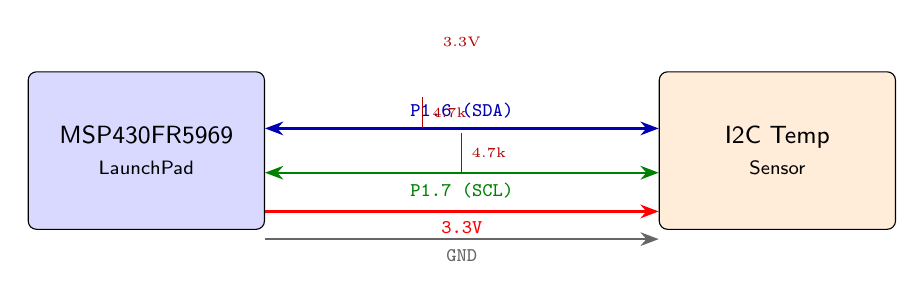
\begin{tikzpicture}[
    box/.style={draw, rounded corners=3pt, minimum height=2cm,
                minimum width=3cm, align=center, font=\small\sffamily},
    >=Stealth
  ]

  % MCU and Sensor
  \node[box, fill=blue!15] (mcu) {MSP430FR5969\\{\scriptsize LaunchPad}};
  \node[box, fill=orange!15, right=5cm of mcu] (sensor) {I2C Temp\\{\scriptsize Sensor}};

  % Signal lines
  \draw[<->, thick, blue!70!black]
    ([yshift=8pt]mcu.east) -- node[above, font=\scriptsize\ttfamily] {P1.6 (SDA)}
    ([yshift=8pt]sensor.west);
  \draw[<->, thick, green!50!black]
    ([yshift=-8pt]mcu.east) -- node[below, font=\scriptsize\ttfamily] {P1.7 (SCL)}
    ([yshift=-8pt]sensor.west);

  % Pull-ups
  \node[font=\tiny, text=red!70!black, above=1.2cm of mcu.east, xshift=2.5cm]
    (vcc) {3.3V};
  \draw[red!70!black] ([yshift=8pt, xshift=2cm]mcu.east) --
    ++(0,0.4) node[midway, right, font=\tiny] {4.7k};
  \draw[red!70!black] ([yshift=-8pt, xshift=2.5cm]mcu.east) --
    ++(0,0.5) node[midway, right, font=\tiny] {4.7k};

  % Power
  \draw[->, thick, red]
    ([yshift=-22pt]mcu.east) -- node[below, font=\scriptsize\ttfamily] {3.3V}
    ([yshift=-22pt]sensor.west);
  \draw[->, thick, black!60]
    ([yshift=-32pt]mcu.east) -- node[below, font=\scriptsize\ttfamily] {GND}
    ([yshift=-32pt]sensor.west);

\end{tikzpicture}
\end{center}

\vspace{0.3em}
\begin{columns}[T]
\begin{column}{0.48\textwidth}
\begin{block}{Common I2C Connections}
\begin{tabular}{@{}ll@{}}
\textbf{LaunchPad} & \textbf{Sensor} \\
P1.6 (J1 pin 10) & SDA \\
P1.7 (J1 pin 9)  & SCL \\
3.3V              & VDD \\
GND               & GND + addr pins \\
\end{tabular}
\end{block}
\end{column}
\begin{column}{0.48\textwidth}
\begin{block}{Supported Sensors}
\scriptsize
\begin{tabular}{@{}lll@{}}
\textbf{Sensor} & \textbf{Addr} & \textbf{Addr Pins} \\
MCP9808 & \texttt{0x18} & A0,A1,A2$\to$GND \\
ADT7410 & \texttt{0x48} & A0,A1$\to$GND \\
\end{tabular}

\vspace{0.3em}
\normalsize
Pull-ups: 4.7\,k$\Omega$ on SDA/SCL to 3.3V
(most breakouts include these).
Same wiring for both sensors.
\end{block}
\end{column}
\end{columns}
\end{frame}

% ---------------------------------------------------------------------------
\begin{frame}[fragile]{MCP9808 vs ADT7410: Register Comparison}
\begin{table}
\centering
\small
\begin{tabular}{@{}lll@{}}
\toprule
& \textbf{MCP9808 (Microchip)} & \textbf{ADT7410 (Analog Devices)} \\
\midrule
I2C Address   & \texttt{0x18} (A0=A1=A2=GND) & \texttt{0x48} (A0=A1=GND) \\
Temp Register & \texttt{0x05} & \texttt{0x00} \\
Resolution    & 0.0625\,\textdegree C (13-bit) & 0.0625\,\textdegree C (13-bit default) \\
Range         & $-40$ to $+125$\,\textdegree C & $-40$ to $+150$\,\textdegree C \\
ID Register   & \texttt{0x06}=0x0054 (mfr) & \texttt{0x0B}=0xCB (8-bit) \\
              & \texttt{0x07}=0x04xx (dev) & upper 5 bits = mfr ID \\
Supply        & 2.7--5.5\,V & 2.7--5.5\,V \\
\bottomrule
\end{tabular}
\end{table}

\vspace{0.3em}
\begin{columns}[T]
\begin{column}{0.48\textwidth}
\begin{block}{MCP9808 Temp Format}
\scriptsize
Upper byte: [7:5] alerts, [4] sign, [3:0] int\\
Lower byte: [7:4] int, [3:0] frac (1/16\,\textdegree C)\\
Sign bit in upper byte bit 4
\end{block}
\end{column}
\begin{column}{0.48\textwidth}
\begin{block}{ADT7410 Temp Format}
\scriptsize
16-bit register, bits [15:3] = temperature\\
Bits [2:0] = status flags\\
Bit 15 = sign (two's complement)
\end{block}
\end{column}
\end{columns}

\vspace{0.3em}
\begin{alertblock}{Same Resolution}
Both sensors use 0.0625\,\textdegree C per LSB, so the fractional
display logic is identical --- only parsing differs.
\end{alertblock}
\end{frame}

% ---------------------------------------------------------------------------
\begin{frame}[fragile]{Example: SPI Flash Read}
\begin{lstlisting}[style=cstyle,
  title={SPI flash read --- W25Q SPI flash memory}]
#define FLASH_CS_LOW()   do { P3OUT &= ~BIT0; } while(0)
#define FLASH_CS_HIGH()  do { P3OUT |=  BIT0; } while(0)
#define FLASH_CMD_READ   0x03

static void flash_read(uint32_t addr, uint8_t *buf, uint16_t len)
{
    tiku_spi_config_t cfg = {
        .mode      = TIKU_SPI_MODE_0,
        .bit_order = TIKU_SPI_MSB_FIRST,
        .prescaler = TIKU_BOARD_SPI_BRW_2MHZ
    };
    uint8_t cmd[4];

    tiku_spi_init(&cfg);

    /* Build 4-byte read command: opcode + 24-bit address */
    cmd[0] = FLASH_CMD_READ;
    cmd[1] = (uint8_t)(addr >> 16);
    cmd[2] = (uint8_t)(addr >> 8);
    cmd[3] = (uint8_t)(addr);

    FLASH_CS_LOW();
    tiku_spi_write(cmd, 4);      /* Send command + address */
    tiku_spi_read(buf, len);     /* Clock out data (sends 0xFF) */
    FLASH_CS_HIGH();

    tiku_spi_close();
}
\end{lstlisting}
\end{frame}

% ---------------------------------------------------------------------------
\begin{frame}[fragile]{Example 10: I2C Temp Sensor Process (examples/10\_i2c\_temp/)}
\begin{lstlisting}[style=cstyle, basicstyle=\ttfamily\tiny,
  title={Periodic I2C temperature read --- sensor selected at compile time}]
static struct tiku_timer poll_timer;
TIKU_PROCESS(temp_sensor_process, SENSOR_NAME);  /* "MCP9808" or "ADT7410" */

TIKU_PROCESS_THREAD(temp_sensor_process, ev, data)
{
    static tiku_i2c_config_t i2c_cfg;
    static int16_t temp_int;
    static uint8_t temp_frac, temp_neg;

    TIKU_PROCESS_BEGIN();
    tiku_common_led1_init();
    tiku_common_led2_init();

    /* Init I2C at 100 kHz, verify sensor identity */
    i2c_cfg.speed = TIKU_I2C_SPEED_STANDARD;
    tiku_i2c_init(&i2c_cfg);
    if (!sensor_verify_id()) {      /* Checks MCP9808 or ADT7410 IDs */
        tiku_i2c_close();
        TIKU_PROCESS_EXIT();
    }

    tiku_timer_set_event(&poll_timer, 2 * TIKU_CLOCK_SECOND);

    while (1) {
        TIKU_PROCESS_WAIT_EVENT_UNTIL(ev == TIKU_EVENT_TIMER);

        if (sensor_read_temp(&temp_int, &temp_frac, &temp_neg)
            == TIKU_I2C_OK) {
            int frac = (int)((uint16_t)temp_frac * 625 / 100);
            TIKU_PRINTF("[%s] Temp: %s%d.%d C\n", SENSOR_NAME,
                        temp_neg ? "-" : "", (int)temp_int, frac);
            tiku_common_led1_toggle();
        }
        tiku_timer_reset(&poll_timer);
    }
    TIKU_PROCESS_END();
}
TIKU_AUTOSTART_PROCESSES(&temp_sensor_process);
\end{lstlisting}
\end{frame}

% ===========================================================================
\section{File Organization}
% ===========================================================================

\begin{frame}[fragile]{Bus Interface Module Files}
\begin{table}
\centering
\small
\begin{tabular}{@{}llp{5.5cm}@{}}
\toprule
\textbf{Layer} & \textbf{File} & \textbf{Role} \\
\midrule
\multirow{2}{*}{I2C API}
  & \texttt{interfaces/bus/tiku\_i2c\_bus.h} & Public types \& prototypes \\
  & \texttt{interfaces/bus/tiku\_i2c\_bus.c} & Validation, delegates to arch \\
\midrule
\multirow{2}{*}{SPI API}
  & \texttt{interfaces/bus/tiku\_spi\_bus.h} & Public types \& prototypes \\
  & \texttt{interfaces/bus/tiku\_spi\_bus.c} & Validation, delegates to arch \\
\midrule
HAL
  & \texttt{hal/tiku\_i2c\_hal.h} & Routes to I2C arch \\
  & \texttt{hal/tiku\_spi\_hal.h} & Routes to SPI arch \\
\midrule
\multirow{2}{*}{Arch (MSP430)}
  & \texttt{arch/msp430/tiku\_i2c\_arch.c/.h}  & eUSCI\_B0 I2C master \\
  & \texttt{arch/msp430/tiku\_spi\_arch.c/.h}  & eUSCI\_A1 SPI master \\
\midrule
\multirow{2}{*}{Board Config}
  & \texttt{.../tiku\_device\_fr5969.h}  & eUSCI availability flags \\
  & \texttt{.../tiku\_board\_fr5969\_launchpad.h}  & Pin select \& prescaler macros \\
\midrule
Example
  & \texttt{examples/10\_i2c\_temp/}  & I2C temp sensor (MCP9808/ADT7410) \\
\bottomrule
\end{tabular}
\end{table}
\end{frame}

% ===========================================================================
\section{Summary}
% ===========================================================================

\begin{frame}{Summary}
\begin{columns}[T]
\begin{column}{0.48\textwidth}
\begin{block}{I2C Bus}
\begin{itemize}
  \item 2-wire (SDA + SCL) via eUSCI\_B0
  \item 100\,kHz standard / 400\,kHz fast
  \item 3 operations: write, read, write\_read
  \item NACK detection + timeout guards
  \item Auto STOP on every error path
\end{itemize}
\end{block}

\begin{block}{SPI Bus}
\begin{itemize}
  \item 3-wire + CS via eUSCI\_A1
  \item All 4 SPI modes, MSB/LSB order
  \item 4 operations: transfer, write, read, write\_read
  \item Application-managed CS via GPIO
  \item Up to 4\,MHz from 8\,MHz SMCLK
\end{itemize}
\end{block}
\end{column}

\begin{column}{0.48\textwidth}
\begin{block}{Architecture}
\begin{itemize}
  \item Platform-independent API in \texttt{interfaces/bus/}
  \item HAL routing in \texttt{hal/}
  \item MSP430 arch in \texttt{arch/msp430/}
  \item Board macros for pin config \& clock
  \item Same arch code works across all FR variants
\end{itemize}
\end{block}

\begin{block}{FR5969 LaunchPad Module Assignment}
\begin{tabular}{@{}ll@{}}
eUSCI\_A0 & UART (backchannel) \\
eUSCI\_A1 & SPI \\
eUSCI\_B0 & I2C \\
eUSCI\_B1 & (available) \\
\end{tabular}
\end{block}
\end{column}
\end{columns}
\end{frame}

% ---------------------------------------------------------------------------
\begin{frame}{Thank You}
\begin{center}
\Large\textbf{TikuOS Bus Interfaces}\\[0.5em]
\normalsize I2C \& SPI for Physical AI Endpoints\\[1.5em]

\begin{tabular}{rl}
  Repository: & \url{https://github.com/tikuos/tikuOS} \\
  License:    & Apache 2.0 \\
  I2C API:    & \texttt{interfaces/bus/tiku\_i2c\_bus.h} \\
  SPI API:    & \texttt{interfaces/bus/tiku\_spi\_bus.h} \\
  I2C Arch:   & \texttt{arch/msp430/tiku\_i2c\_arch.c} \\
  SPI Arch:   & \texttt{arch/msp430/tiku\_spi\_arch.c} \\
\end{tabular}
\end{center}
\end{frame}

\end{document}
